%%%%%%%%%%%%%%%%%%%%%%%%%%%%%%%%%%%%%%%%%%%%%%%%%%%%%%%%%%%%%%%%%%%%%
% LaTeX Template: Project Titlepage Modified (v 0.1) by rcx
%
% Original Source: http://www.howtotex.com
% Date: February 2014
% 
% This is a title page template which be used for articles & reports.
% 
% This is the modified version of the original Latex template from
% aforementioned website.
% 
%%%%%%%%%%%%%%%%%%%%%%%%%%%%%%%%%%%%%%%%%%%%%%%%%%%%%%%%%%%%%%%%%%%%%%

\documentclass[a4paper,11pt]{report}
\usepackage[parfill]{parskip}
%\usepackage[default]{lato}
%\usepackage{kpfonts}%  for math    
\usepackage{libertine}%  serif and sans serif
%\usepackage[scaled=0.85]{beramono}%% mono

\usepackage[T1]{fontenc}
\usepackage[utf8]{inputenc}
\usepackage[a4paper]{geometry}
\usepackage[toc]{glossaries}
\usepackage[myheadings]{fullpage}
\usepackage{fancyhdr}
\usepackage{lastpage}
\usepackage{graphicx, wrapfig, caption, subcaption, setspace, booktabs}
\usepackage[font=small, labelfont=bf]{caption}
\usepackage{fourier}
\usepackage[protrusion=true, expansion=true]{microtype}
\usepackage[english]{babel}
\usepackage{sectsty}
\usepackage{url, lipsum}
\usepackage{enumitem}
\usepackage{amsmath}
\usepackage{float}
\usepackage[numbers]{natbib}
%\usepackage[round]{natbib}

\usepackage[english]{babel}

\usepackage{hyperref}
\hypersetup{
	colorlinks,
	citecolor=black,
	filecolor=black,
	linkcolor=black,
	urlcolor=black
}
%\pagenumbering{roman}

\newcommand{\HRule}[1]{\rule{\linewidth}{#1}}
\onehalfspacing
\setcounter{tocdepth}{3}
\setcounter{secnumdepth}{3}
\renewcommand{\baselinestretch}{1.1}

%-------------------------------------------------------------------------------
% HEADER & FOOTER
%-------------------------------------------------------------------------------
\pagestyle{fancy}
\fancyhf{}
\setlength\headheight{15pt}
\fancyhead[L]{Medical Sensors Report}
\fancyhead[R]{University of Burgundy}
%\fancyfoot[R]{Page \thepage\ of \pageref{LastPage}}
\fancyfoot[C]{\thepage}
%\pagenumbering{roman}
%-------------------------------------------------------------------------------
% TITLE PAGE
%-------------------------------------------------------------------------------
% abbreviations:
\newacronym{ny}{NY}{New York}
\newacronym{la}{LA}{Los Angeles}
\newacronym{un}{UN}{United Nations}
\newacronym{dwt}{DWT}{Discrete Wavelet Transform}
\newacronym{ft}{FT}{Fourier Transform}


% nomenclature:
\newglossaryentry{angelsperarea}{
  name = $a$ ,
  description = The number of angels per unit area,
}
\newglossaryentry{numofangels}{
  name = $N$ ,
  description = The number of angels per needle point
}
\newglossaryentry{areaofneedle}{
  name = $A$ ,
  description = The area of the needle point
}

\makeglossaries

\DeclareMathOperator*{\argmin}{argmin} 
\DeclareMathOperator*{\argmax}{argmax}  

\begin{document}
	
	
\title{ \textsc{\textbf{Medical Sensors}}
		\\ [0.5cm] 
		\normalsize \textsc{Project Report}
		\\
		[2.0cm]
		\HRule{0.5pt} \\
		\LARGE \textbf{PET/CT Image Denoising and Segmentation based on a Multi Observation and Multi Scale Markov Tree Model}
		\HRule{2pt} \\ [0.5cm]
		\normalsize \today \vspace*{5\baselineskip}}

\date{}

\author{
		Yeman Hagos \\
		Vu Hoang Minh \\ }

\maketitle
\tableofcontents
\newpage

%-------------------------------------------------------------------------------
% Section title formatting
\sectionfont{\scshape}
%-------------------------------------------------------------------------------

%-------------------------------------------------------------------------------
% BODY
%-------------------------------------------------------------------------------

%Chapter 1 - introduction
%---------------------------------------------------------------------------------
\chapter{Introduction}
\label{chap:introduction}
Image denoising and segmentation are essential step in many advanced techniques of image processing. 

Image noise is a random variation of brightness and visible as grains. It may arise
by the sensor and circuity of a digital camera during the time of capturing or image
transmission that adds spurious and extraneous information \cite{verma2013comparative}. Noise in image
is defined as pixels showing false or different intensity values instead of true or
expected values. Natural image denoising is a process of reducing or removing
noise from an image. In other words, it is defined as a process of estimating an
original clean version of noise corrupted image \cite{levin2011natural}.

 According to actual image characteristic, noise statistical property and frequency spectrum distribution rule, people have developed many methods of eliminating noises, which approximately are divided into space and transformation fields. the transformations generate some coefficients  and then  processed. Then the aim of eliminating noise is achieved by inverse transformation, like wavelet transform and contourlet transforms \cite{ruikar2011wavelet}\cite{matalon2005image}.Wavelet denoising attempts to remove the noise present in the signal while preserving the signal characteristics, regardless of its frequency content \cite{rangarajan2002image}.

Image segmentation is an important early vision task where pixels with similar features are grouped into homogeneous regions in which  class labels are assigned to each pixels in the image according to the properties of a pixel and neighborhood pixels. It is a joint process of detection and estimation of class labels to each pixels and shapes of homogeneous regions. 

These days, Bayesian estimation has become popular method to study the statistical properties of regions of an image to determine the possible number of class labels and to assign pixels to the corresponding label. Most of Bayesian techniques use region models to describe statistics of homogeneous regions of an image. The \gls{mrf} has been extensively in use to model the class labels of the pixels in the image. The image is segmented by estimating the\gls{map}  or\gls{ml} estimate of the pixels\cite{choi1999image} \cite{voisin2014supervised}.

In this paper, we implemented  multi-observation and multi resolution  denoising (contourlet and wavelet) and segmentation tumor in \gls{cti} and \gls{pet} images.

The paper is organized as follows. In Chapter 2, we introduced about \gls{wt}, \gls{ct}, \gls{wd}, \gls{cd}, \gls{wcd}, and \gls{hmt}. Chapter 3 gives the implementation and algorithm of our decisioning and segmentation. Section IV gives the developed method overview. In Chapter 4, we present the denoising and segmentation of CT and PET images, and discussion. Finally, Chapter 5 presents conclusions our implementation.



%Chapter 2 - literature review
%---------------------------------------------------------------------------------
\chapter{Literature Review}
\label{chap:literature-review}
%---------------------------------------------------------------------------------




\section{HMT}
I am witrh Minh the bitch.
\section{Wavelet Transform}

\subsection{Overview}
Wavelet transforms have become increasingly important in digital signal processing and image processing since wavelets allow both time and frequency analysis simultaneously. The use of wavelets for these purposes is a recent development, although the theory is not new. The principles are similar to those of Fourier analysis, which was first developed in the early part of the 19th century.

In signal processing, wavelets make it possible to recover weak signals from noise . This has proven useful especially in the processing of X-ray and magnetic-resonance images in medical applications. Images processed in this way can be "cleaned up" without blurring or muddling the details.

\subsection{Definition}
A function $\psi \,\in\, L^2(\mathbb{R})$  is called an
orthonormal wavelet if it can be used to define a
, that is a
$L^2\left(\mathbb{R}\right)$ of


\section{Contourlet Transform}

%=====================================================
\subsection{Background}
In the field of Geometrical Image Transforms, there are many 1-D transforms designed for detecting or capturing the geometry of image information, such as the \gls{ft} and \gls{wt}. However, the ability of 1-D transform processing of the intrinsic geometrical structures, such as smoothness of curves, is limited in one direction, then more powerful representations are required in higher dimensions. The \gls{ct}, which was proposed in \cite{do2005contourlet}, is a new two-dimensional transform method for image representations.

Contourlets form a multiresolution directional tight frame designed to efficiently approximate images made of smooth regions separated by smooth boundaries. The \gls{ct} has a fast implementation based on a \gls{lp} decomposition followed by \glspl{dfb} or \glspl{pdfb} applied on each bandpass subband \cite{suresh2014artificial}. The new method as proposed in \cite{lu2006new} uses a multiscale pyramid that can be adjusted by applying low pass or high pass filters for the different levels.

The \gls{lp} decomposition only produce one bandpass image in a multidimensional signal processing, that can avoid frequency scrambling. And \gls{dfb} is only fit for high frequency since it will leak the low frequency of signals in its directional subbands. This is the reason to combine \gls{dfb} with \gls{lp}, which is multiscale decomposition and remove the low frequency.

\begin{figure}[h]
	\centering
	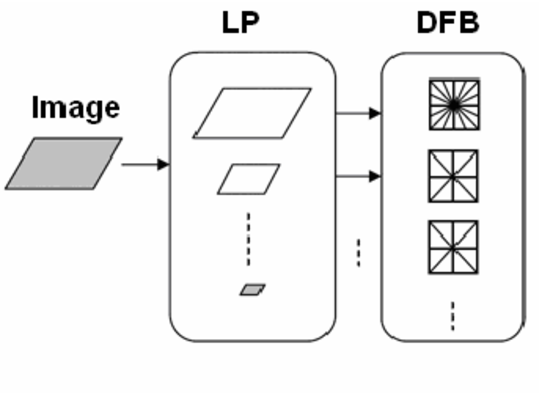
\includegraphics[width=0.7\textwidth]{fig/contourlet}
	\caption[Contourlet Transform - Filter Bank]{Filter Bank}
	\label{fig:contourlet}
\end{figure}


%=====================================================
\subsection{Contourlet Transform}

The \gls{ct} is a directional transform, capable of capturing contours and fine details in images. The Figure \ref{fig:contourlet_2} illustrates the \gls{ct}, in which the input image consists of frequency components like \gls{ll}, \gls{lh}, \gls{hl} and \gls{hh}. 

\begin{figure}[h]
	\centering
	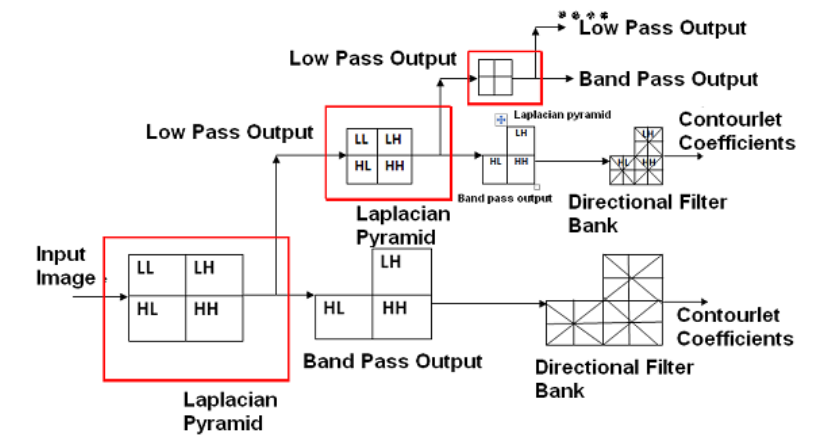
\includegraphics[width=0.7\textwidth]{fig/contourlet_2}
	\caption[Contourlet Transform - Decomposition of Filter Bank]{Decomposition of Filter Bank}
	\label{fig:contourlet_2}
\end{figure}

The \gls{lp} at each level generates a Low pass output (LL) and a Band pass output (LH, HL, and HH). The Band pass output is then passed into \gls{dfb}, which
results in contourlet coefficients. The Low pass output is again passed through the \gls{lp} to obtain more coefficients and this is done till the fine details of the image are obtained. Figure \ref{fig:contourlet_mr} shows the decomposition of brain MR Image. 

\begin{figure}[h]
	\centering
	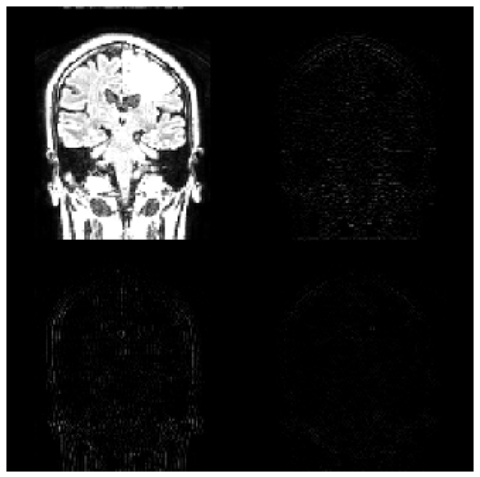
\includegraphics[width=0.45\textwidth]{fig/contourlet_mr}
	\caption[Contourlet Transform - Decomposition of brain MR Image]{Contourlet decomposition of brain MR Image}
	\label{fig:contourlet_mr}
\end{figure}




\section{PET Image Denoising}

%==================================================
\subsection{Image Denoising}
Image noise is a random variation of brightness and visible as grains. It may arise
by the sensor and circuity of a digital camera during the time of capturing or image
transmission that adds spurious and extraneous information \cite{verma2013comparative}. Noise in image
is defined as pixels showing false or different intensity values instead of true or
expected values. Natural image denoising is a process of reducing or removing
noise from an image. In other words, it is defined as a process of guesstimating an
original clean version of noise corrupted image \cite{levin2011natural}.

The common types of noise that arises in a image are impulse noise (salt-and-pepper
noise), amplifier noise (Gaussian noise), shot noise, quantization noise (uniform
noise), film grain, on-isotropic noise, multiplicative noise (speckle noise) and periodic
noise. Depending on owning different characteristics, which makes them
distinguishable, each type of noise is able to afflict image in different context. As
a result, noise reduction filters are developed to minimize the effects of noise in
order to ameliorate image processing.

In paper \cite{hanzouli2013pet}, the developed framework was firstly evaluated for \gls{pet} denoising. In this work the multiobservation
aspect of the proposed \gls{hmt} was exploited in
order to associate both Wavelets and Contourlets coefficients
to each voxel. An approach combining both \gls{cd} and \gls{wd}, namely \gls{wcd}, was proposed in order to obtain the optimal performance.


%==================================================
\subsection{PET Image}
\gls{pet} is a nuclear medicine, functional imaging technique that is used to observe metabolic processes in the body. The system detects pairs of gamma rays emitted indirectly by a positron-emitting radionuclide (tracer), which is introduced into the body on a biologically active molecule. 

Three-dimensional images of tracer concentration within the body are then constructed by computer analysis. In modern PET-CT scanners, three dimensional imaging is often accomplished with the aid of a CT X-ray scan performed on the patient during the same session, in the same machine.

The examples of \gls{pet} system and \gls{pet} brain image can be seen in Figure \ref{fig:pet_image}.

\begin{figure}[h]
	\centering
	\begin{subfigure}[b]{0.45\textwidth}
		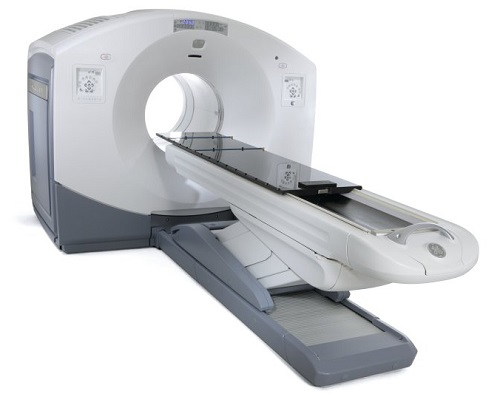
\includegraphics[width=\textwidth]{fig/pet_machine.jpg}
		%\caption{\gls{pet} machine}
		\label{fig:pet_machine}
	\end{subfigure}
	\begin{subfigure}[b]{0.35\textwidth}
		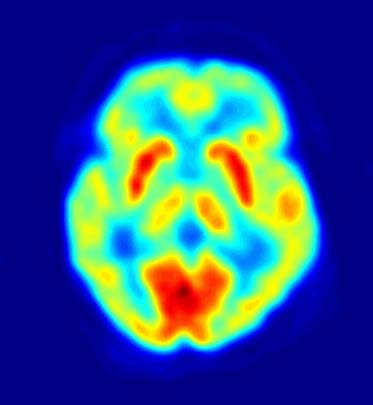
\includegraphics[width=\textwidth]{fig/pet_brain.jpg}
		%\caption{\gls{pet} brain image}
		\label{fig:pet_brain}
	\end{subfigure}
	\caption{\gls{pet} system and \gls{pet} brain image}\label{fig:pet_image}
\end{figure}


%==================================================
\subsection{Wavelet and Contourlet Denoising}
\label{subsection:wavelet_denoising}

%--------------------------------------------------
\subsubsection*{Wavelet denoising}
Wavelet thresholding methods for noise removal, in which the wavelet coefficients are
thresholded in order to remove their noisy part, were first introduced by Donoho in 1993 \cite{coifman1995translation}.
The theoretical justifications and arguments in their favour are highly compelling. These
methods do not require any particular assumptions about the nature of the signal, permits
discontinuities and spatial variation in the signal, and exploits the spatially adaptive
multiresolution of the wavelet transform \cite{cohen2012signal}.

%--------------------------------------------------
\subsubsection*{Contourlet Denoising}
The major drawback for wavelets in two-dimensions is
their limited ability in capturing directional information. To
overcome this deficiency, researchers have recently considered multiscale and directional representations that can capture the
intrinsic geometrical structures such as smooth contours in
natural images \cite{Po2003}.

The primary goal of the contourlet construction is to obtain a sparse expansion for typical images that
are piecewise smooth away from smooth contours \cite{do2005contourlet}.

%--------------------------------------------------
\subsubsection*{Concept of denoising}

\begin{figure}[h]
	\centering
	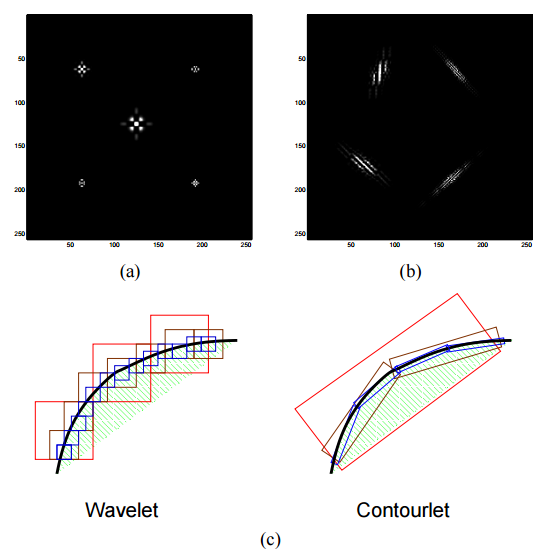
\includegraphics[width=0.7\textwidth]{fig/wavelets_contourlet}
	\caption{Contourlet and wavelet representations for images. (a) Examples of
		five 2-D wavelet basis images. (b) Examples of four contourlet basis images.
		(c) Illustration showing how wavelets having square supports that can only
		capture point discontinuities, whereas contourlets having elongated supports
		that can capture linear segments of contours, and thus can effectively represent
		a smooth contour with fewer coefficients.
	}
	\label{fig:wavelets_contourlet}
	
\end{figure}

A more precise explanation of the wavelet denoising
procedure can be given as follows. Assume that the
observed data is \cite{rangarajan2002image}:
\begin{equation}
X(t)=S(t)+N(t)
\end{equation}
where $S(t)$ is the uncorrupted signal with additive
noise $N(t)$. 

Let $W(\cdot)$ and $W^{-1}(\cdot)$ denote the forward
and inverse wavelet transform operators. Let $D(\cdot, \lambda)$ denote the denoising operator with threshold $\lambda$. 

We intend to denoise $X(t)$ to recover $\hat{S}(t)$ as an estimate
of $S(t)$. The procedure can be summarized in three
steps:
\begin{subequations}
	\begin{align}
	Y &= W(X)\\
	Z &= D(Y,\lambda)\\
	\hat{S} &= W^{-1}(Z)
	\end{align}
	\label{eqn:wavelet_denoise}
\end{subequations}
while $D(\cdot,\lambda)$ being the thresholding operator and $\lambda$ being the threshold.

%--------------------------------------------------
\subsubsection*{Thresholding}
In fact, small coefficients are dominated by noise, while coefficients with a large absolute value carry more signal information than noise. Replacing noisy coefficients (small coefficients below a certain threshold value) by zero and an inverse wavelet transform may lead to a reconstruction that has lesser noise \cite{rangarajan2002image}. 

There are three kinds of thresholding for denoising:
\begin{itemize}
	\item Hard thresholding
	\item Soft thresholding
	\item Universal thresholding
\end{itemize}

\begin{figure}[h]
	\centering
	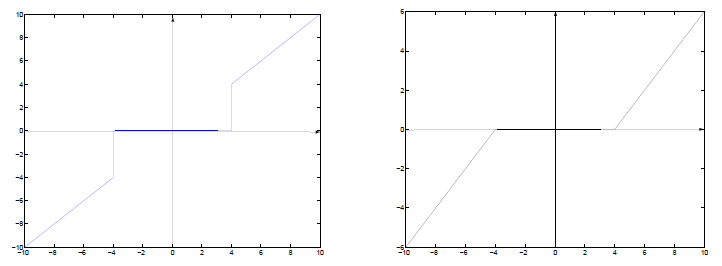
\includegraphics[width=0.8\textwidth]{fig/hard_soft_thresholding}
	\caption{Hard and Soft Thresholding}
	\label{fig:hard_soft_thresholding}
\end{figure}

Hard threshold is a "keep or kill" procedure and
is more intuitively appealing. The alternative, soft
thresholding shrinks coefficients above the threshold in absolute value. See Figure \ref{fig:hard_soft_thresholding} for the transfer functions of hard and soft thresholding, respectively. 

The hard thresholding operator is defined as:
\begin{equation}
D(U, \lambda) = 
\begin{cases}
U &\text{for all $|U|>\lambda$ }\\
0 &\text{otherwise}
\end{cases}	
\end{equation}

Otherwise, the soft thresholding operator is defined as:
\begin{equation}
D(U, \lambda) = sgn(U)max(0, |U| - \lambda)
\end{equation}

Threshold determination is an important question when denoising. A small threshold
may yield a result close to the input, but the
result may still be noisy. A large threshold on the other hand, produces a signal with a large number
of zero coefficients. This leads to a smooth signal.
Paying too much attention to smoothness, however,
destroys details and in image processing may cause
blur and artifacts \cite{rangarajan2002image}.

In addition to hard and soft thresholding, a thresholding approach, namely universal thresholding, is introduced:
\begin{equation}
\lambda_{UNIV}=\sqrt{2lnN\sigma}
\end{equation}
where $N$ being the signal length, and $\sigma^2$ being the noise variance.


%==================================================
\subsection{Wavelet-Contourlet Denoising}

\begin{figure}[h]
	\centering
	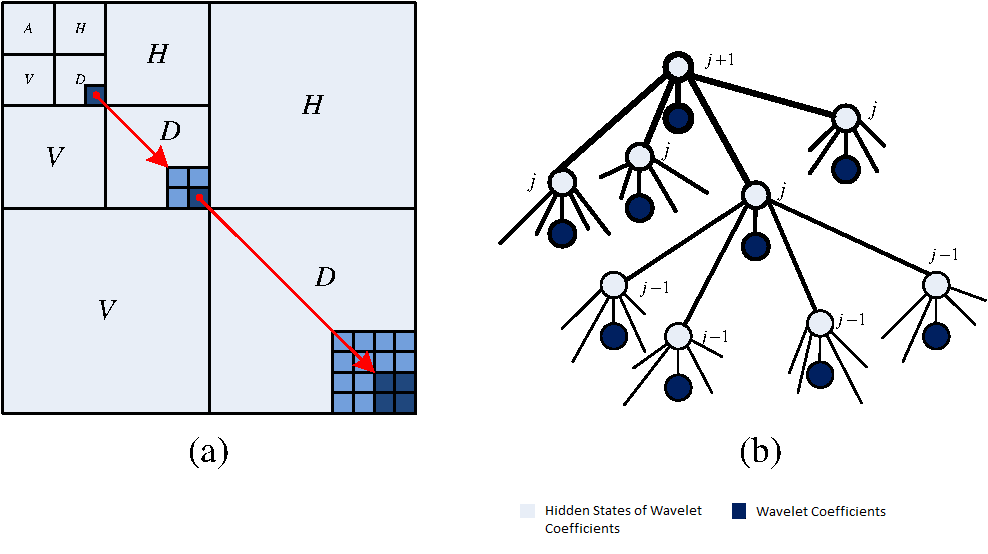
\includegraphics[width=0.8\textwidth]{fig/wavelets_hmt}
	\caption{\glsdesc{dwt} and \glsdesc{hmt} models}
	\label{fig:wavelets_hmt}
\end{figure}


%==================================================
\subsection{Proposed denoising method: Non-local Means}
%--------------------------------------------------
%\subsubsection*{Background}

\gls{nlm} is a linear smoothing technique introduced by \citeauthor{buades2005non}. \gls{nlm} filtering
is an algorithm computing average values of all pixels in the image, which are analyzed
how similar they are to the objective pixel. The main difference between \gls{nlm} and other filters is the meticulous employment of all possible self-predictions
an image is able to provide.

Compared to local filters, which process pixels within a local square window to aim
for a reconstruction of the main geometrical configurations, \gls{nlm} is more effective
in post-filtering intelligibility and preserving details of image and fine structure \cite{buades2005non}.


%==================================================
\subsection{Proposed denoising method: Sparse 3D Transform-domain Collaborative Filter}
%--------------------------------------------------
%\subsubsection*{Background}
Currently, \gls{bm3d} is a well-known
image denoising algorithm introduced by \citeauthor{dabov2007image} in 2007 \cite{dabov2007image}. The basic principles
of this algorithm is grouping and collaborative Wiener filtering in two-stage
estimations. There is a number of developed algorithms based on the concepts of
BM3D; however, BM3D is still the most successful
approach, especially for low-SNR \gls{pet} image.



%\footnote{An example footnote.}
\section{PET/CT Image Segmentation}

\subsection{Introduction}
Segmentation is the process of splitting an observed image into its homogeneous or constituent regions . Segmentation may also be thought of as labeling process, where each pixel in a given image is assigned a designating the region or class to which it belongs. If the observed image y is defined on a rectangular $M \times N$ lattice $\Omega$, indexed  by a pair $(i,j)$ so that \(\Omega={(i,j);1\leq i\leq M and 1 \leq j \leq N}\) and the label x will be defined on the same label. Thus for each pixel site $s=(s_i,s_j)$ there is a label $x_s$ which specifies to which region the pixel $y_s$ belongs. The relationship between  gray scale values and levels is represented by Bayesian Likelihood function.  It is modeled by probability distribution of the pixel values, model parameter and the prior distribution of models. Then segmentation is an optimization problem  of the labels on entire image\cite{barker1998image}.

Graph partitioning methods are an effective tools for image segmentation since they model the impact of pixel neighborhoods on a given cluster of pixels or pixel, under the assumption of homogeneity in images. In these methods, the image is modeled as a weighted, undirected graph. Usually a pixel or a group of pixels are associated with nodes and edge weights define the (dis)similarity between the neighborhood pixels. The graph (image) is then partitioned according to a criterion designed to model "good" clusters. Each partition of the nodes (pixels) output from these algorithms are considered an object segment in the image.\par
MRFs are completely characterized by their prior probability distributions, marginal probability distributions, cliques, smoothing constraint as well as criterion for updating values. The criterion for image segmentation using MRFs is restated as finding the labeling scheme which has maximum probability for a given set of features. \par

In terms of image segmentation, the function that MRFs seek to maximize is the probability of identifying a labeling scheme given a particular set of features are detected in the image




where Vc(x) is the clique potential and C is the set of all possible cliques. In the image domain, we assume that one pixel has at most 4 neighbors: the pixels in its 4-neighborhood. Then the clique potential is defined on pairs of neighboring pixels
%http://www.cs.cmu.edu/~16831-f14/notes/F11/16831_lecture07_bneuman.pdf

The HMRF-EM framework was first proposed for segmentation of brain MR images [9]. Given an image \(Y=(y_1, y_2,..., y_N)\) where each \(y_i\) is the intensity of a pixel, we want to infer a configuration of labels\(X = (x_1,x_2,...,x_N)\) where\(x_i \in L\)  and L is the set of all possible labels which means the hidden process is a finite valued one(REFERENCE:IMAGE AND SIGNAL RESTORATION USING PAIRWISE MARKOV TREES) In a binary segmentation problem, L = \{0,1\} . According to the MAP criterion, we seek the labeling \(x^*\) which satisfies:
\begin{equation}
X^*=\argmax_x\{\Pr( Y \mid X, \Theta)P(X)\} 
\end{equation}
The prior probability \(P(X)\) is a Gibbs distribution, and the joint likelihood probability is given by:

\begin{equation}\label{eq1}
\begin{split}
\Pr( Y \mid X,\Theta) & =\prod_{i}^{ }\Pr( y_i \mid X,\Theta)\\
& =\prod_{i}^{ }\Pr( y_i \mid X_i,\theta_{x_i})
\end{split}
\end{equation}

where \[Pr( y_i \mid X_i,\theta_{x_i})\] is a Gaussian distribution with parameters
\(\theta_{x_i}=(\mu_{x_i} , \sigma_{x_i})\) and \(\Theta=\{\theta_l\lvert l \in L\}\)
is the parameter set,which is obtained by the EM algorithm.

\subsection{EM Algorithm}
We use the EM algorithm to estimate the parameter set \(\Theta=\{\theta_l\lvert l \in L\}\). We describe the EM algorithm by the following \cite{bordes2007stochastic}:

\begin{enumerate}
	\item Start: Assume we have an initial parameter set\(\Theta^{(0)}\)
	\item  E-step: At the \(t^th\) iteration, we have  \(|\Theta^{(t)}\) and we calculate the conditional expectation:
\end{enumerate}
\begin{equation}
Q(\Theta \mid \Theta^{(t)}) = {\sum\limits_{x} }\Pr( x \mid Y,\Theta^{(t)})\ln (\Pr( x,Y \mid \Theta))
\end{equation}
where $ x \in X$, set of all possible configurations of labels.

\begin{enumerate}
	\setcounter{enumi}{2}
	\item M-step: Now maximize \(\Pr(\Theta \mid \Theta^{(t)})\) to obtain the next
	estimate:
\end{enumerate}
\begin{equation}
\Theta^{(t+1)}==\argmax_x\{\Pr(\Theta \mid \Theta^{(t)})\} 
\end{equation}
Then let \(\Theta^{(t+1)}\) to \(\Theta^{(t)}\) and repeat from the E-step.

The above equations are in general are computationally difficult and here we have assumed the parameters are random processes to simplify our implementation\cite{monfrini2003image}. Let \(G(z;\theta_l)\) denote a Gaussian distribution function with parameters \(\theta_l=(\mu_l,\sigma_l)\):
\begin{equation}
G(z;\theta_l)= \frac{1}{\sqrt{2\pi\sigma^2}}\exp(-\frac{(z-\mu_l)^2}{2\sigma^2})   
\end{equation}
We assume that the prior probability can be written as:
\begin{equation}
P(X)=\frac{1}{Z}\exp{(-U(X))}  
\end{equation}
where U(X) is the prior energy function. We also assume that


\begin{equation}\label{eq2}
\begin{split}
\Pr( Y \mid X,\Theta) & =\prod_{i=1}^{ }\Pr( y_i \mid x_i,\Theta_{x_i})\\
& =\prod_{i}^{ }G(y_i;\theta_{x_i})\\
& =\frac{1}{Z'}\exp{(-U(Y \mid X)} 
\end{split}
\end{equation}

With these assumptions, the HMRF-EM algorithm is given below:

\begin{enumerate}
	\item Start with initial parameter set \(\Theta^{(0)}\).
	\item Calculate the likelihood distribution \(P^{(t)}(y_i \mid x_i,\theta_{x_i})\).
	\item Using current parameter set \(\Theta^{(t)}\) to estimate the labels
	by MAP estimation:
\end{enumerate}

\begin{equation}
\begin{split}
X^{(t)} & =\argmax_{x \in X}\{\Pr( Y \mid X, \Theta^{(t)})P(X)\}\\
&= \argmin_{x \in X} \{U( Y \mid X, \Theta^{(t)}) + U(X)\}
\end{split}
\end{equation}
The algorithm for the MAP estimation is discussed below.

\begin{enumerate}
	\setcounter{enumi}{3}
	\item Calculate the posterior distribution for all  \(l \in L\) and  all pixels \(y_i\):
\end{enumerate}
\begin{equation}
\Pr^{(t)}(l \mid y_i)=\frac{G(y_i;\theta_i)Pr(l \mid x^{(t)}_{N_i})}{P^{(t)(y_i)}}
\end{equation}
where \(x^{(t)}_{N_i}\) is the neighborhood configuration of \(x^{(t)}_i\)
and
\begin{equation}
P^{(t)}(y_i)={\sum\limits_{l \epsilon L} }G(y_i;\theta_i)Pr(l \mid x^{(t)}_{N_i})
\end{equation}

Note here we have

\begin{equation}
Pr(l \mid x^{(t)}_{N_i})=\frac{1}{Z}\exp(-{\sum\limits_{j \epsilon N_i}}V_c(l,x^t_j))
\end{equation}

\begin{enumerate}
	\setcounter{enumi}{4}
	\item Use \(P^{(t)}(l \mid y_i)\) to update the parameters: 
\end{enumerate}

\begin{equation}
\begin{split}
\mu^{(t+1)}_l & = \frac{{\sum\limits_{i}}P^{(t)}(l \mid y_i)y_i}{{\sum\limits_{i}}P^{(t)}(l \mid y_i)} \\
(\sigma^{(t+1)}_l)^2 & =\frac{{\sum\limits_{i}}P^{(t)}(l \mid y_i)(y_i-\mu^{t+1}_l)^2}{{\sum\limits_{i}}P^{(t)}(l \mid y_i)}
\end{split}
\end{equation}

\subsection{MAP Estimation}
In the EM algorithm, we need to solve for x? that minimizes
the total posterior energy
\begin{equation}\label{eq:MAp}
X^* = \argmin_{x \in X} \{U( Y \mid X, \Theta) + U(X)\}
\end{equation}
with given $Y$ and $\Theta$, where the likelihood energy is

\begin{equation}
\begin{split}
U( Y \mid X, \Theta) & ={\sum\limits_{i}}U( Y_i \mid X_i, \Theta)\\
& = {\sum\limits_{i}}(\frac{(y_i-\mu_{x_i})^2}{2\sigma_{x_i}^2} + \ln(\sigma_{x_i}))
\end{split}
\end{equation}

The prior energy function U(x) has the form
\begin{equation}
U(X) = {\sum\limits_{c \epsilon C}}V_c(X)
\end{equation}
where $V_c(X)$ is the clique potential and C is the set of all
possible cliques.

In the image domain, we assume that one pixel has at most 4 neighbors: the pixels in its 4-neighborhood. Then the clique potential is defined on pairs of neighboring pixels:

\begin{equation}
V_c(x_i,x_j) = \frac{1}{2}(1-I_{x_i,x_i})
\end{equation}
Where
\begin{equation}
I_{x_i,x_i}=
\begin{cases} 
0 & \text{if } x_i\neq x_j \\
1      & \text{if } x_i= x_j 
\end{cases}
\end{equation}

We have developed an iterative algorithm to solve (\ref{eq:MAp}):


\begin{enumerate}
	\item To start with, we have an initial estimate \(X^(0)\), which is from the previous loop of the EM algorithm. 
	\item Provided \(X^{(k)}\), for all \(1\leq i \leq N\), we find
\end{enumerate}

\begin{equation}
X^{(k+1)}_i=\argmin_{l \in L} \{U( y_i \mid l) + {\sum\limits_{j \epsilon N_i}}V_c(l,x^k_j))\}
\end{equation}

\begin{enumerate}
	\item Repeat step 2 until \(U( Y \mid X, \Theta) + U(X)\) converges or a maximum k is achieved.
\end{enumerate}





%Chapter 3 - implementation
%---------------------------------------------------------------------------------
\chapter{Implementation}
\label{chp:implementation}
%---------------------------------------------------------------------------------

%---------------------------------------------------------------------------------%

\section{Coding Standard}

%Chapter 4 - result
%---------------------------------------------------------------------------------
\chapter{Result and Discussion}
\label{chap:result}
%--------------------------------------------------------------------
We applied the contourlet HMT model for denoising and texture retrieval, and obtained promising results.

Two example are illustrated in Figure \ref{fig:petct1} and \ref{fig:petct2} as below:

\begin{figure}[h]
	\centering
	\begin{subfigure}{.5\textwidth}
		\centering
		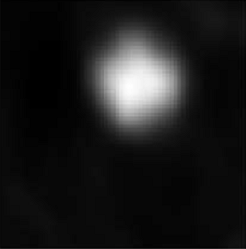
\includegraphics[width=.8\linewidth]{fig/pet1}
		\caption{PET image}
		\label{fig:sub1}
	\end{subfigure}%
	\begin{subfigure}{.5\textwidth}
		\centering
		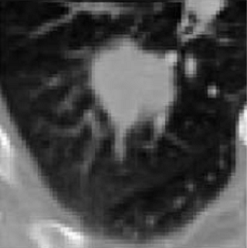
\includegraphics[width=.8\linewidth]{fig/ct1}
		\caption{CT Image}
		\label{fig:sub2}
	\end{subfigure}
	\caption{PET and CT images}
	\label{fig:petct1}
\end{figure}

\begin{figure}[h]
	\centering
	\begin{subfigure}{.5\textwidth}
		\centering
		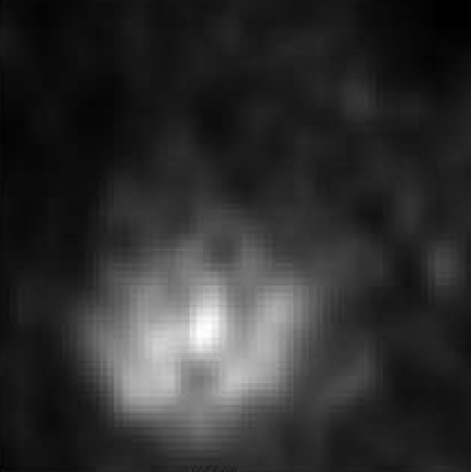
\includegraphics[width=.8\linewidth]{fig/pet2}
		\caption{PET image}
		\label{fig:sub1}
	\end{subfigure}%
	\begin{subfigure}{.5\textwidth}
		\centering
		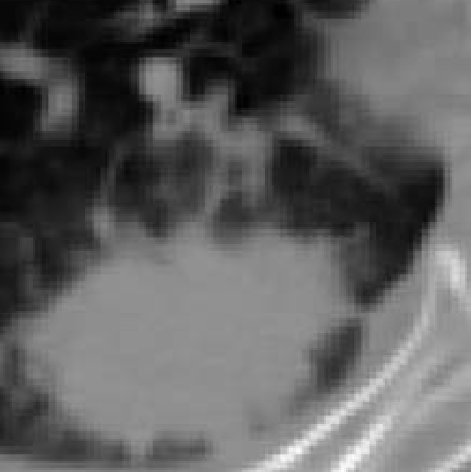
\includegraphics[width=.8\linewidth]{fig/ct2}
		\caption{CT Image}
		\label{fig:sub2}
	\end{subfigure}
	\caption{PET and CT images}
	\label{fig:petct2}
\end{figure}


In denoising, the \gls{ct} visually restores edges better than wavelet and other classical methods. It capture directional information well and offer a valuable tool in image processing. 

On the other hand, Wavelet based methods exploit observation-based transforms at different resolutions in order to better describe the whole observed information . The major drawback of Wavelets is their limited ability in capturing directional information. Consequently, an approach combining both transforms may lead to optimal performance. Our implementation combines this two methods and we achieved promising results.


The selection of the denoising technique is application dependent. So, it is necessary
to learn and compare denoising techniques to select the technique that is apt for the
application in which we are interested. By far there is no criterion of image quality evaluation that can be accepted generally
by all. A technique to calculate the signal to noise ratio in images has been proposed
which can be used with some approximation.

In this project, we have used Wavelet-Contourlet and BM3D for denoising purpose. The results can be shown in Figure \ref{fig:de1} and Figure \ref{fig:de2}. 




\begin{figure}[h]
	\centering
	\begin{subfigure}{.5\textwidth}
		\centering
		
\includegraphics[width=.8\linewidth]{fig/wavelet}
		\caption{Wavelet Denoising}
		\label{fig:sub1}
	\end{subfigure}%
	\begin{subfigure}{.5\textwidth}
		\centering
		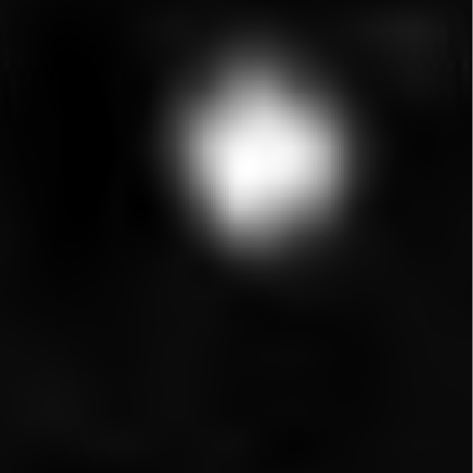
\includegraphics[width=.8\linewidth]{fig/contourlet.jpg}
		\caption{Contourlet Denoising}
		\label{fig:sub2}
	\end{subfigure}
	\caption{Wavelet and Contourlet Denoising}
	\label{fig:de1}
\end{figure}

\begin{figure}[h]
	\centering
	\begin{subfigure}{.5\textwidth}
		\centering
		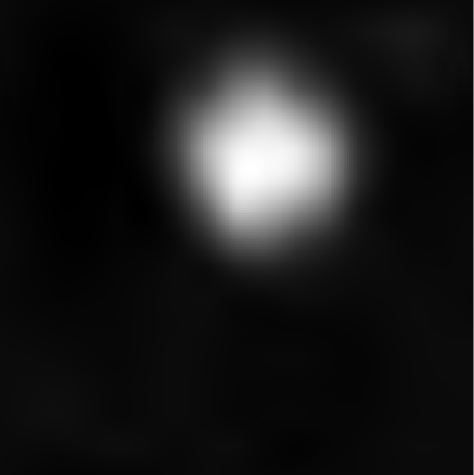
\includegraphics[width=.8\linewidth]{fig/wavecon}
		\caption{Wavelet Denoising}
		\label{fig:sub1}
	\end{subfigure}%
	\begin{subfigure}{.5\textwidth}
		\centering
		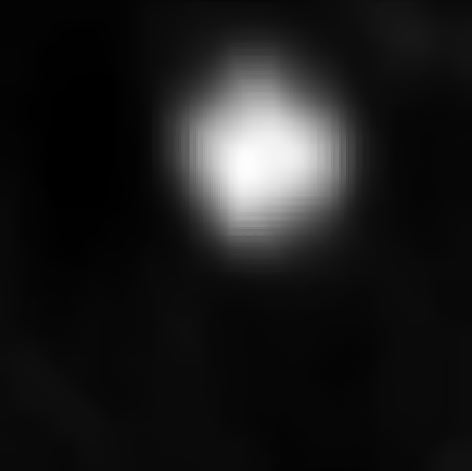
\includegraphics[width=.8\linewidth]{fig/bm3d.jpg}
		\caption{Contourlet Denoising}
		\label{fig:sub2}
	\end{subfigure}
	\caption{Wavelet-Contourlet and BM3D Denoising}
	\label{fig:de2}
\end{figure}


Image registration is the process of transforming different sets of data into one coordinate system.   It is alignment of one image
 with another. Images may be of same or different types (MR, CT, PET)

 
 In Medical imaging no single image modality provides a complete picture in all cases. Images of different modalities will infer a more comprehensive story than provided by either. So,  fusion of different modality is needed. In our implementation we have used a manual image registration using Matlab. 
 
 
 Figure \ref{fig:seg1} and \ref{fig:seg2} shows the segmented images of PET and CT.
 

 
\begin{figure}[h]
	\centering
	\begin{subfigure}{.5\textwidth}
		\centering
		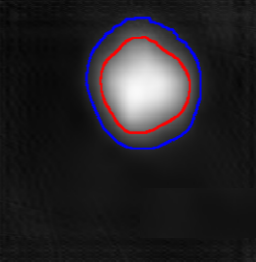
\includegraphics[width=.8\linewidth]{fig/pet1_marked}
		\caption{Segmented PET image}
		\label{fig:sub1}
	\end{subfigure}%
	\begin{subfigure}{.5\textwidth}
		\centering
		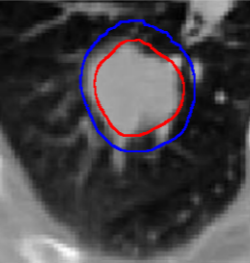
\includegraphics[width=.8\linewidth]{fig/ct1_marked}
		\caption{Segmented CT Image}
		\label{fig:sub2}
	\end{subfigure}
	\caption{PET and CT images}
	\label{fig:seg1}
\end{figure}

\begin{figure}[h]
	\centering
	\begin{subfigure}{.5\textwidth}
		\centering
		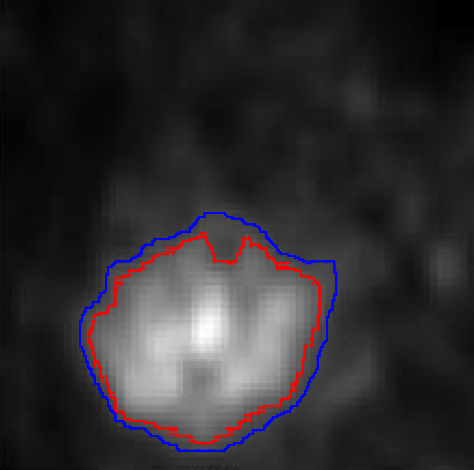
\includegraphics[width=.8\linewidth]{fig/pet2_marked}
		\caption{Segmented PET image}
		\label{fig:sub1}
	\end{subfigure}%
	\begin{subfigure}{.5\textwidth}
		\centering
		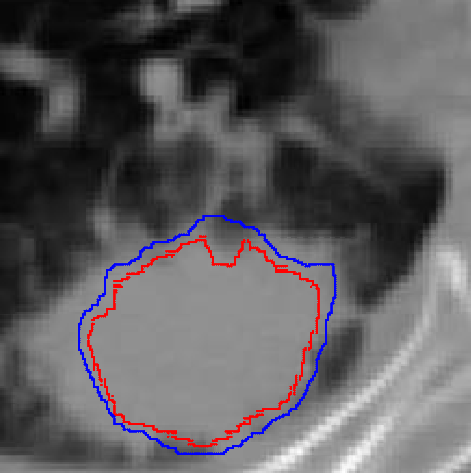
\includegraphics[width=.8\linewidth]{fig/ct2_marked}
		\caption{Segmented CT Image}
		\label{fig:sub2}
	\end{subfigure}
	\caption{PET and CT images}
	\label{fig:seg2}
\end{figure}

 In conclusion, we achieved the same results compared to the Paper.

%Chapter 5 - conclusion
%---------------------------------------------------------------------------------
\chapter{Conclusion}
\label{chap:conclusion}

%--------------------------------------------------------------------
In this project we have implemented \textbf{PET/CT Image Denoising and Segmentation based on a Multi Observation and a Multi Scale Markov Tree Model}. We have applied wavelet and contourlet transforms to denoise the image to utilize the advantage of both methods. For co segmentation of PET and CT images must be aligned first. Thus, we applied image registration . Finally, Segmentation was performed on PET and CT images using HMT. Our implementation gave us an excellent result of detecting tumors on both PET and CT images.

For the future, we would like to apply our algorithm on PET-MRI and MRI images, and work on enhancing the segmentation algorithm by integrating HMT  with evidence theory and neural network.




%-------------------------------------------------------------------------------
% REFERENCES
%-------------------------------------------------------------------------------
\newpage
%\section*{References}
\bibliography{ref} 
%\bibliographystyle{plainnat}
\bibliographystyle{ieeetr}

\end{document}